% Copyright 2026 Sreeram Anil
% SPDX-License-Identifier: CC-BY-4.0
% =============================================================================
%  Baseline methods — chapter order
%
%  Reading order:
%    1. Coulomb counting: the ampere-hour integral. Perfect dynamics, no
%       feedback; its error is a closed-form function of the sensor calibration
%       and the capacity error, and that formula is the yardstick for every
%       "current-bias" and "aged-cell" result in the rest of the report.
%    2. OCV inversion: the dual failure. No memory, no drift, but an error
%       equal to the voltage-model error divided by the OCV slope.
%    3. The industrial hybrid: Coulomb counting pulled towards the IR/RC-compensated
%       OCV inversion whenever the load drops below 0.3 C (60 s time constant).
%       It beats both of its parents and shows what a scheduled gain buys.
%
%  These three are not competitive estimators and are not presented as such.
%  They are the two error mechanisms that every model-based filter in Parts
%  III-X exists to trade off against each other, in their pure form.
% =============================================================================
% Copyright 2026 Sreeram Anil
% SPDX-License-Identifier: CC-BY-4.0
% =============================================================================
%  Coulomb counting (ampere-hour integration) — baseline family
% =============================================================================
\chapter{Coulomb Counting (ampere-hour integration)}
\label{ch:coulombcounting}

\section*{At a glance}
\begin{tabular}{@{}l>{\raggedright\arraybackslash}p{0.76\textwidth}@{}}
Family & baselines \\
Header & \texttt{include/estkit/battery/baselines.hpp} \\
Registered name & \texttt{CoulombCounting} \\
State dimension & $n_x = 4$ propagated open-loop; only $\soc$ is reported \\
Cost per step & $\mathcal{O}(n_x)$, $\approx 79$\,ns/step measured, no heap, no feedback \\
Primary references & \cite{ng2009coulomb,plett2015bms1,lin2018sensorbias} \\
\end{tabular}

\section{Motivation and relevance}
Coulomb counting is the open-loop integration of the measured current, and it is worth studying in
its pure form for three reasons. It is the \emph{time update} of every Kalman filter in
Parts~III--VI --- the $\soc$ row of the ECM model (Chapter~\ref{ch:ecm}) is exactly
\eqref{eq:cc-recursion}, so whatever afflicts it also afflicts the EKF's prediction step; the
difference is only that a filter gets to correct it. Its error is \emph{analytic}: alone among the
methods in this report, its end-of-mission error is a closed-form function of the current-sensor
gain and offset, the elapsed time, the throughput and the capacity error, and \eqref{eq:cc-drift}
is the quantitative baseline for the \code{current\_bias} and \code{aged\_cell} columns of every
results table. And it is the fallback when a voltage channel fails or the cell sits on an OCV
plateau, so a certification argument needs a defensible statement about it. Ng
et~al.~\cite{ng2009coulomb} made the essential point --- the practical limit is sensor calibration
and capacity knowledge, not the integration --- and it is why no production BMS ships it alone.

\section{Problem statement and assumptions}
The method estimates only $\soc$, from the current channel; the voltage is accepted and ignored, and
a predicted voltage is reported so that the residual diagnostic of \S\ref{sec:me-residual} is
available.
\begin{assumption}\label{as:cc-all}
(i) the capacity $Q$ is known and constant; (ii) the current sensor is calibrated,
$i^{\text{m}} = i$ up to zero-mean noise; (iii) $\hat\soc_0 = \soc_0$.
\end{assumption}
All three are violated by the benchmark on purpose. Item~(iii) is the sharpest: there is no
feedback, so an initial error is never removed.

\section{Derivation}
With the discharge-positive convention, coulombic efficiency $\eta(i)=1$ on discharge and $\eta_c$
on charge, and a zero-order hold on the current over $[t_{k-1},t_k)$,
\begin{equation}
\hat\soc_{k} \;=\; \hat\soc_{k-1} \;-\; \frac{\eta(i^{\text{m}}_{k-1})\,\dt}{3600\,\hat Q}\; i^{\text{m}}_{k-1},
\label{eq:cc-recursion}
\end{equation}
$\hat Q$ being the capacity in \si{\ampere\hour} the estimator was told. The implementation obtains
this by calling the model's $f$, so $v_1,v_2,h$ propagate open-loop alongside $\soc$ and make the
diagnostic voltage $\hat v_k = h(\xminus_k,\vu_k)$ meaningful.

Let $e_k = \hat\soc_k - \soc_k$, let the true capacity be $Q = \hat Q(1-\delta)$ with $\delta$ the
fractional capacity loss, and let the current channel be $i^{\text{m}} = \kappa i + b_i + n_k + q_k$
(gain, offset, noise, quantisation residual; Chapter~\ref{ch:datasets}). Integrating
\eqref{eq:cc-recursion} over a mission of duration $T$ with throughput
$A_h = \frac{1}{3600}\int_0^T i\,\mathrm{d}t$ in \si{\ampere\hour}, and subtracting the true
evolution $\soc(T)-\soc(0) = -A_h/Q$, gives
\begin{equation}
\boxed{\;
e(T) \;=\; \underbrace{e(0)}_{\text{initial}}
\;-\;\underbrace{\frac{(\kappa-1)\,A_h}{\hat Q}}_{\text{gain}}
\;-\;\underbrace{\frac{b_i\,T/3600}{\hat Q}}_{\text{offset}}
\;-\;\underbrace{\frac{\mathcal{N}}{\hat Q}}_{\text{noise}}
\;+\;\underbrace{\frac{A_h\,\delta}{\hat Q(1-\delta)}}_{\text{capacity}} \; }
\label{eq:cc-drift}
\end{equation}
with $\mathcal{N} = \frac{1}{3600}\int_0^T(n+q)\,\mathrm{d}t$. Four consequences follow.

\emph{Gain scales with throughput, offset with time.} A \SI{19}{\minute} hover-hold and a
\SI{48}{\minute} fixed-wing mission remove almost the same charge, so their gain-induced errors are
equal, but the offset term is $2.5\times$ larger on the longer one. A sensor specified only by its
full-scale accuracy cannot be assessed without the duty cycle.

\emph{The random part is negligible.} $\mathcal{N}$ is a random walk of standard deviation
$\sigma_i\sqrt{\dt\,T}/3600 = \SI{1.97e-4}{\ampere\hour}$ over the eVTOL mission --- \SI{0.004}{\percent}
of SOC, two orders below the deterministic terms --- and quantisation adds
$q_i/\sqrt{12} = \SI{2.9}{\milli\ampere}$~\cite{widrow2008quantization} and a further
\SI{0.0002}{\percent}. Ampere-hour integration does not accumulate sensor noise; it accumulates
sensor \emph{bias}. The only quantisation mechanism that matters is the degenerate one, where a
constant current sits at a fixed distance from a code boundary and the rounding residual becomes a
DC offset of up to $q_i/2 = \SI{5}{\milli\ampere}$, worth \SI{0.056}{\percent} of SOC per mission.

\emph{The capacity term has the dangerous sign.} It is positive for $\delta>0$: an aged cell, whose
true capacity is smaller than the estimator believes, yields an estimate that is too \emph{high}.
Coulomb counting on an aged cell is systematically optimistic --- the failure direction that matters
on final approach. When $\delta$ accumulates during the mission as $\delta\propto A_h^{z}$ with
$z=0.55$, the integral replaces the product and the term becomes $\delta A_h/\bigl((1+z)\hat Q\bigr)$.

\emph{There is no forgetting.} $e(0)$ appears with coefficient one for all $T$, so
\code{init\_error} is not a convergence test for this method but a demonstration that it has no
convergence.

\paragraph{Quantitative check.} Substituting the nominal eVTOL numbers
($A_h = \SI{3.763}{\ampere\hour}$, $T=\SI{2010}{\second}$, $\hat Q = \SI{5}{\ampere\hour}$,
$\kappa = 1.005$, $b_i = \SI{20}{\milli\ampere}$, in-flight fade $\delta = \SI{0.327}{\percent}$)
into \eqref{eq:cc-drift} gives $-0.376-0.223+0.159 = -\SI{0.44}{\percent}$, against a measured final
error of $-\SI{0.443}{\percent}$. For \code{current\_bias} it predicts
$-1.505-2.792+0.159 = -\SI{4.14}{\percent}$ against a measured $e_{\max}$ of \SI{4.14}{\percent};
for \code{aged\_cell}, $-0.60+13.28 = +\SI{12.7}{\percent}$ against \SI{12.90}{\percent}. The formula
is not an approximation of the benchmark --- it \emph{is} the benchmark.

\section{Algorithm, application and implementation}
\begin{algorithm}[H]
\caption{Coulomb counting --- one sampling period}
\begin{algorithmic}[1]
\Require $\xhat_{k-1}$, stored $\vu_{k-1}$, new $i^{\text{m}}_k, T^{\text{m}}_k$ ($v^{\text{m}}_k$ unused)
\State $\vu_k \gets [\,i^{\text{m}}_k,\ T^{\text{m}}_k\,]^\T$
\If{$k>0$} \State $\xhat_k \gets f(\xhat_{k-1},\vu_{k-1})$ \Comment{open-loop; the $\soc$ row is \eqref{eq:cc-recursion}}
\EndIf
\State $\hat v_k \gets h(\xhat_k,\vu_k)$ \Comment{diagnostic only; never fed back}
\State $\vu_{k-1}\gets\vu_k$
\Ensure $\hat\soc_k = \xhat_k[\soc]$
\end{algorithmic}
\end{algorithm}

There is no tuning: the estimator uses \code{params} and \code{z0} from \code{EstimatorConfig} and
ignores $\mQ$, $\mR$ and $\sigma_{\soc_0}$ because it has no covariance; $\eta_c = 0.995$ acts only
on charge. The step is four multiply--accumulates, three exponentials (inherited from the shared
$f$) and one OCV lookup for the diagnostic voltage: \SI{79}{\nano\second}, the cheapest estimator in
the library. \code{sizeof} is \SI{4184}{\byte}, of which \SI{3872}{\byte} is the OCV
table used only for the diagnostic --- drop it and the method reduces to four scalars. The float32
build reproduces the double build to five digits; the one numerical caveat is long-horizon
accumulation, since over the 120-flight protocol the estimator performs $6\times10^{7}$ additions
and in binary32 a running sum near \num{0.5} absorbing increments of $10^{-5}$ is at the edge of
resolution. Compensated (Kahan) summation is the standard remedy and is not implemented because the
double build does not need it.

\section{Benchmark results}
% Copyright 2026 Sreeram Anil
% SPDX-License-Identifier: CC-BY-4.0
\begin{table}[H]\centering\footnotesize\setlength{\tabcolsep}{4pt}
\caption{CoulombCounting: cell-level benchmark on the eVTOL mission (mean over seeds; RMSE and max error in \% SOC; $t_\mathrm{conv}$: first time the error stays below 2\,\% for 60\,s, -- = never; EKF reference: steady-state RMSE of the plain EKF on the same data).}\label{tab:cell_CoulombCounting}
\begin{tabular}{llrrrrrcrr}\toprule
plant & scenario & RMSE & RMSE$_\mathrm{ss}$ & max & $t_\mathrm{conv}$ [s] & RMSE$_v$ [mV] & div. & EKF ref. & ns/step \\ \midrule
ECM & nominal & 0.28 & 0.36 & 0.44 & 0 & 3.41 & no & 0.05 & 79 \\
ECM & init\_error & 35.25 & 35.35 & 35.44 & -- & 8153.93 & yes & 0.05 & 79 \\
ECM & current\_bias & 2.44 & 3.20 & 4.14 & 0 & 28.12 & no & 0.61 & 81 \\
ECM & noise\_step & 0.28 & 0.36 & 0.44 & 0 & 3.41 & no & 0.12 & 80 \\
ECM & outliers & 0.28 & 0.35 & 0.44 & 0 & 3.39 & no & 0.21 & 80 \\
ECM & cold & 0.34 & 0.44 & 0.56 & 0 & 6.18 & no & 0.16 & 79 \\
ECM & hot & 0.20 & 0.24 & 0.28 & 0 & 2.25 & no & 0.03 & 80 \\
ECM & aged\_cell & 7.80 & 10.05 & 12.90 & 0 & 112.49 & no & 1.52 & 79 \\
ECM & param\_mismatch & 0.28 & 0.36 & 0.44 & 0 & 16.24 & no & 1.36 & 80 \\
ECM & sensor\_dropout & 0.28 & 0.36 & 0.44 & 0 & 3.41 & no & 0.46 & 79 \\
ECM & preisach & 0.28 & 0.36 & 0.44 & 0 & 9.24 & no & 0.20 & 80 \\
ECM & combined & 22.19 & 20.94 & 25.04 & -- & 1543.50 & no & 12.44 & 79 \\
\midrule
SPM & nominal & 0.36 & 0.47 & 0.60 & 0 & 10.26 & no & 3.73 & 75 \\
SPM & init\_error & 35.32 & 35.46 & 35.60 & -- & 8157.11 & yes & 3.81 & 75 \\
SPM & current\_bias & 2.52 & 3.31 & 4.30 & 0 & 29.47 & no & 5.69 & 75 \\
SPM & noise\_step & 0.36 & 0.47 & 0.60 & 0 & 10.26 & no & 3.30 & 74 \\
SPM & outliers & 0.36 & 0.46 & 0.60 & 0 & 10.24 & no & 1.99 & 74 \\
SPM & cold & 0.36 & 0.47 & 0.60 & 0 & 37.77 & no & 7.35 & 75 \\
SPM & hot & 0.36 & 0.47 & 0.60 & 0 & 8.84 & no & 2.16 & 73 \\
SPM & param\_mismatch & 0.36 & 0.47 & 0.60 & 0 & 18.69 & no & 3.13 & 75 \\
SPM & sensor\_dropout & 0.36 & 0.47 & 0.60 & 0 & 10.26 & no & 5.31 & 75 \\
\bottomrule\end{tabular}\end{table}

\begin{figure}[H]\centering
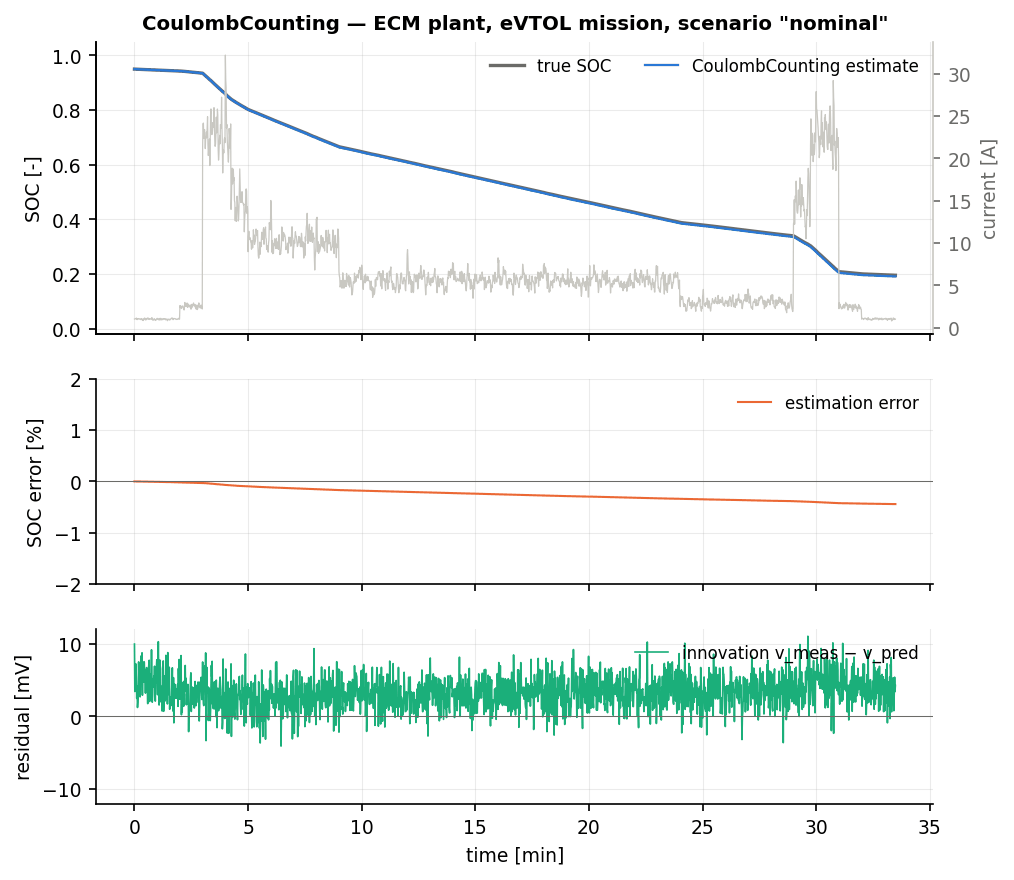
\includegraphics[width=0.78\textwidth]{figures/cell_CoulombCounting_nominal.png}
\caption{Coulomb counting on the nominal eVTOL mission: true and estimated SOC (top), estimation
error (middle), voltage residual (bottom). The error is a smooth monotone ramp --- the integral of a
constant bias --- with no visible noise-driven component, as \eqref{eq:cc-drift} predicts.}
\end{figure}
\begin{figure}[H]\centering
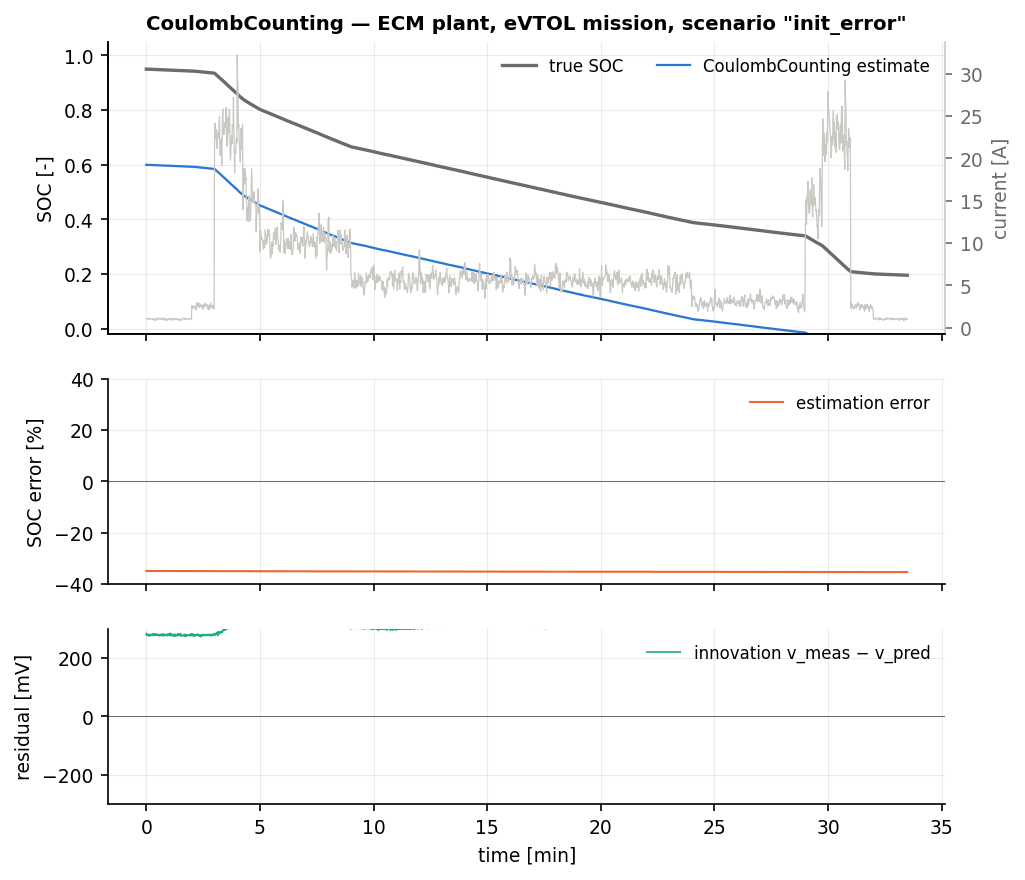
\includegraphics[width=0.78\textwidth]{figures/cell_CoulombCounting_init_error.png}
\caption{Coulomb counting with a $-35\,\%$ initial SOC error: the error is carried, unchanged, to
the end of the mission.}
\end{figure}

On the nominal eVTOL mission the method achieves $\text{RMSE}=0.28\,\%$ and
$\text{RMSE}_{\text{ss}}=0.36\,\%$ --- seven times the EKF's $0.05\,\%$, but in absolute terms
\SI{18}{\milli\ampere\hour} on a \SI{5}{\ampere\hour} cell. The steady-state figure \emph{exceeds}
the whole-run figure because the error grows monotonically; this inversion of the usual ordering is
the fingerprint of an uncorrected integrator, and it is the single clearest discriminator in the
whole results set --- every estimator with a working measurement update shows
$\text{RMSE}_{\text{ss}} \le \text{RMSE}$ on this scenario.

The scenarios split into three groups. Those that leave the current and the capacity alone ---
\code{noise\_step}, \code{outliers}, \code{sensor\_dropout}, \code{param\_mismatch} and
\code{preisach} --- give an estimate bit-identical to nominal ($0.36\,\%$ in every case, $0.35\,\%$
for \code{outliers}), because the voltage is not used. This is the one context in which the method
wins outright: $0.36\,\%$ against the EKF's $0.46\,\%$ on \code{sensor\_dropout}, against
$1.36\,\%$ on \code{param\_mismatch} and against the hybrid's $2.28\,\%$ on \code{preisach}
(Chapter~\ref{ch:coulombocvhybrid}). An estimator that does not look cannot be deceived. The
voltage-residual column still moves ($3.41\to\SI{16.24}{\milli\volt}$ under \code{param\_mismatch},
\SI{9.24}{\milli\volt} under \code{preisach}) --- a useful demonstration that $\text{RMSE}_v$
diagnoses the \emph{model} independently of the state.

Those touching the current channel or the capacity fail exactly as \eqref{eq:cc-drift} says:
\code{current\_bias} $3.20\,\%$ ($5.2\times$ the EKF), \code{aged\_cell} $10.05\,\%$ ($6.6\times$),
\code{init\_error} $35.35\,\%$ with a divergence flag, \code{combined} $20.94\,\%$. The
$\text{RMSE}_v$ column is the tell in each case --- \SIlist{28;112}{\milli\volt}, then
\SIlist{8.15;1.54}{\volt} --- so a supervisory function monitoring the residual would detect every
one of these failures within seconds even though the estimator cannot.

The temperature scenarios are counter-intuitive: \code{hot} \emph{improves} the result to
$0.24\,\%$ and \code{cold} degrades it to $0.44\,\%$. Neither has anything to do with the
integration; temperature enters \eqref{eq:cc-drift} only through the capacity-fade term, and at
\SI{45}{\celsius} the Arrhenius ageing rate is higher, so $\delta$ grows faster and the positive
capacity term cancels more of the negative sensor terms. The same accidental cancellation flatters
several estimators in the \code{hot} column throughout this report.

\paragraph{The SPM plant.} On the electrochemical plant the estimators are handed a 2-RC circuit
fitted to it with a \SI{4}{\milli\volt} structured residual (Chapter~\ref{ch:spm}), and Coulomb
counting is the one method in this report that is completely indifferent to that: it never evaluates
the measurement model, so its only sensitivity to the plant is through the lithium bookkeeping,
which is identical in both. Every SPM row is therefore $0.47\,\%$ --- \code{nominal},
\code{noise\_step}, \code{cold}, \code{hot}, \code{param\_mismatch} and \code{sensor\_dropout}
alike, to two decimals --- with only \code{current\_bias} ($3.31\,\%$) and \code{init\_error}
($35.46\,\%$) differing, exactly as \eqref{eq:cc-drift} requires. The comparison that matters is
with the EKF, which scores \numrange{3.73}{7.35}\,\% on the same rows: Coulomb counting beats it on
every SPM scenario except \code{current\_bias}, because the EKF is being corrected by a voltage
model that is wrong by \SI{4}{\milli\volt} RMS and dutifully biases $\soc$ to explain it. The
$\text{RMSE}_v$ column shows the structural error directly --- \SI{10.26}{\milli\volt} on
\code{nominal} against \SI{3.41}{\milli\volt} on the ECM plant, and \SI{37.77}{\milli\volt} on
\code{cold}, where the fitted circuit cannot represent the solid-diffusion overpotential at all.
This is the most important negative result of the baseline part: a measurement update improves an
estimate only if the measurement model is better than the prediction model.

\section{Summary}
Use Coulomb counting as the prediction step of something else, as a fallback when the voltage
channel is untrustworthy, and as the analytic yardstick \eqref{eq:cc-drift} when specifying a
current sensor. Do not use it alone over a mission long enough for
$(\kappa-1)A_h + b_iT/3600$ to exceed the accuracy budget --- about \SI{35}{\minute} at a
\SI{0.5}{\percent} budget for this benchmark's nominal sensor --- and never where the capacity is
not tracked independently, because the capacity term is both the largest and the optimistic one. Its
virtue is that its failure is completely predictable, and at \SI{79}{\nano\second} there is no
reason not to run it alongside the real estimator as a cross-check.

% Copyright 2026 Sreeram Anil
% SPDX-License-Identifier: CC-BY-4.0
% =============================================================================
%  OCV inversion (voltage lookup) — baseline family
% =============================================================================
\chapter{Open-Circuit-Voltage Inversion (OCV Lookup)}
\label{ch:ocvlookup}

\section*{At a glance}
\begin{tabular}{@{}l>{\raggedright\arraybackslash}p{0.76\textwidth}@{}}
Family & baselines \\
Header & \texttt{include/estkit/battery/baselines.hpp} \\
Registered name & \texttt{OCVLookup} \\
State dimension & $n_x = 4$; $\soc$ replaced each step, $v_1,v_2,h$ propagate open-loop \\
Cost per step & $\mathcal{O}(n_b)$ with $n_b=40$ bisection steps, $\approx 1310$\,ns/step, no heap \\
Primary references & \cite{plett2015bms1,weng2014ocv,hu2012comparative} \\
\end{tabular}

\section{Motivation and relevance}
Coulomb counting integrates and therefore drifts; the natural complement is a method with no memory
at all --- invert the cell's equilibrium characteristic and read the state of charge off the
terminal voltage. The two fail in exactly opposite ways, and it is the pairing that motivates every
model-based filter in this report: a Kalman filter is precisely a rule for weighting a drift-free
but noisy voltage inversion against a smooth but drifting ampere-hour integral, with the weight
computed from the two error covariances.

The difficulty is that the open-circuit voltage is not measurable in flight. The terminal voltage
during a \SI{22.5}{\ampere} hover differs from the OCV by more than \SI{0.4}{\volt}, against an OCV
span of \SI{1.3}{\volt} over the whole SOC range, so a voltage-lookup method is really a model-based
\emph{overpotential-compensation} method and its numbers are best read as a measurement of the
ECM's fidelity. Its relevant property for an aircraft is the one Coulomb counting lacks: bounded
error. After a reset, a lost non-volatile store or a mid-flight power cycle, the estimate returns to
within the model error in a time set by one filter constant --- a certification-friendly property,
and the reason it survives in production systems as a re-initialisation path.

\section{Problem statement}
The measurement model of Chapter~\ref{ch:ecm} is
\begin{equation}
v \;=\; \ocv(\soc,T) \;+\; M h \;-\; v_1 \;-\; v_2 \;-\; R_0(T)\,i ,
\label{eq:ocv-meas}
\end{equation}
with $v_1,v_2$ the RC overpotentials, $h\in[-1,1]$ the hysteresis state and $M$ its magnitude.
\begin{assumption}\label{as:ocv-all}
(i) $\ocv(\cdot,T)$ is strictly monotone in $\soc$, so $\ocv^{-1}$ exists; (ii) $R_0(T)$, $R_j$,
$\tau_j$, $M$ are known and $v_1,v_2,h$ can be reconstructed from the current history alone;
(iii) $\soc$ varies slowly compared with the low-pass constant $\tau_{\text{lp}}$.
\end{assumption}
Item~(i) holds for this cell but only just --- the slope falls to \SI{0.197}{\volt} near
$\soc=0.90$. Item~(ii) is what \code{param\_mismatch}, \code{cold} and \code{preisach} test; item
(iii) is what fails during the hovers.

\section{Derivation}
Rearranging \eqref{eq:ocv-meas} for the compensated open-circuit voltage,
\begin{equation}
\widehat{\ocv}_k \;=\; v^{\text{m}}_k + R_0(T^{\text{m}}_k)\, i^{\text{m}}_k
 + \hat v_{1,k} + \hat v_{2,k} - M\,\hat h_k ,
\label{eq:ocv-compensate}
\end{equation}
where $\hat v_1,\hat v_2,\hat h$ come from propagating the model's $f$ open-loop with the measured
current --- the same recursion Coulomb counting uses, but here only the overpotential states are
kept and $\soc$ is overwritten each step. The instantaneous SOC is
$\hat\soc^{\text{inst}}_k = \ocv^{-1}(\widehat{\ocv}_k, T^{\text{m}}_k)$, computed by 40 bisection
steps on $[-0.05,1.05]$ against the 241-point table, which resolves the interval to
$1.1/2^{40}\approx10^{-12}$. Bisection rather than Newton is used because it needs no derivative,
cannot diverge, and has a data-independent trip count (\S\ref{sec:lib-mcu}).

This inherits the full voltage noise amplified by the inverse slope, so a first-order low-pass with
$\tau_{\text{lp}} = \SI{30}{\second}$ is applied:
\begin{equation}
\hat\soc_k \;=\; a\,\hat\soc_{k-1} + (1-a)\,\hat\soc^{\text{inst}}_k,
\qquad a = e^{-\dt/\tau_{\text{lp}}} = 0.99667 .
\label{eq:ocv-lowpass}
\end{equation}
Its noise rejection is $\sqrt{\dt/(2\tau_{\text{lp}})} = 0.041$ in standard deviation: a
\SI{2}{\milli\volt} voltage noise over a \SI{0.8}{\volt} slope is \SI{0.25}{\percent} of SOC per
sample, filtered to \SI{0.010}{\percent}. That is the noise floor; everything else is bias.

Linearising the inversion about the true SOC, the estimate error is the compensated-voltage error
divided by the OCV slope:
\begin{equation}
\boxed{\;
\hat\soc^{\text{inst}} - \soc \;=\;
\frac{\delta v + \delta R_0\, i + \delta v_1 + \delta v_2 - M\,\delta h}{\partial\ocv/\partial\soc}
\;+\;\mathcal{O}\!\left(\tfrac{\partial^2\ocv}{\partial\soc^2}\right) \; }
\label{eq:ocv-error}
\end{equation}
Three consequences dominate the benchmark.

\emph{The slope is the gain, and it collapses on the plateau.} For this NMC811/graphite cell
$\partial\ocv/\partial\soc$ is \SIrange{0.71}{1.16}{\volt} over most of $[0.2,0.85]$, so a
\SI{10}{\milli\volt} model error costs about \SI{1.2}{\percent} of SOC; but between $\soc=0.86$ and
$0.93$ the two-phase behaviour of the graphite electrode flattens the curve to \SI{0.197}{\volt} at
$\soc\approx0.895$, where the same error costs \SI{5.1}{\percent}. Every mission starts at
$\soc_0=0.95$ and falls through this plateau in its first minutes.

\emph{The low-pass converts a rate into a bias.} Applying \eqref{eq:ocv-lowpass} to a truth ramping
at $\dot\soc$ gives a steady-state lag
\begin{equation}
\hat\soc - \soc \;\longrightarrow\; -\tau_{\text{lp}}\,\dot\soc \;=\; +\,\frac{\tau_{\text{lp}}\,i}{3600\,Q},
\label{eq:ocv-lag}
\end{equation}
positive on discharge --- the estimate is stale and therefore too high. At the eVTOL cruise
($i=\SI{5.5}{\ampere}$) this is \SI{0.92}{\percent}; during the \SI{22.5}{\ampere} hover,
\SI{3.75}{\percent}. This single term explains the shape of the nominal error trace and is the
method's central tension: $\tau_{\text{lp}}$ must be large to reject noise through a slope gain of
$1/0.2$ to $1/1.2$, and small to avoid lag, and no value is good at both. A filter that weights the
two information sources by their covariances is not a refinement of this method --- it is the
resolution of this dilemma.

\emph{Model error enters multiplied by the current.} $\delta R_0\,i$ is \SI{22.5}{\milli\volt} for a
\SI{1}{\milli\ohm} resistance error at hover, i.e.\ \SI{2.8}{\percent} of SOC at a \SI{0.8}{\volt}
slope; at \SI{-10}{\celsius}, where $R_0$ is \SI{35.1}{\milli\ohm}, the same \emph{relative} error
costs three times as much.

\section{Algorithm}
\begin{algorithm}[H]
\caption{OCV inversion with IR/RC compensation --- one sampling period}
\begin{algorithmic}[1]
\Require $\hat\soc_{k-1}$, overpotential states $\hat v_{1},\hat v_{2},\hat h$, stored $\vu_{k-1}$, new $i^{\text{m}}_k, v^{\text{m}}_k, T^{\text{m}}_k$
\State $\vu_k \gets [\,i^{\text{m}}_k,\ T^{\text{m}}_k\,]^\T$
\If{$k>0$} \State $\xhat \gets f(\xhat,\vu_{k-1})$ \Comment{open-loop RC and hysteresis states}
\EndIf
\State $\hat v_k \gets h(\xhat,\vu_k)$ \Comment{diagnostic voltage prediction}
\State $\widehat{\ocv} \gets v^{\text{m}}_k + R_0(T^{\text{m}}_k)\,i^{\text{m}}_k + \hat v_1 + \hat v_2 - M\hat h$
\State $\hat\soc^{\text{inst}} \gets$ \textbf{bisect} $\ocv(\cdot,T^{\text{m}}_k) = \widehat{\ocv}$ on $[-0.05,1.05]$, 40 steps
\State $\hat\soc_k \gets a\,\hat\soc_{k-1} + (1-a)\,\hat\soc^{\text{inst}}$
\State $\xhat[\soc] \gets \hat\soc_k$; \quad $\vu_{k-1}\gets\vu_k$
\Ensure $\hat\soc_k$
\end{algorithmic}
\end{algorithm}
Line~8 writes the filtered SOC back into the model state, which acts only through the
current-dependence of the hysteresis rate and is second order.

\section{Application and implementation notes}
$\tau_{\text{lp}} = \SI{30}{\second}$ is the only tuning constant, fixed for all scenarios. The
bisection bracket matches the model's \code{constrain} bounds, so the estimate is clamped to the
physical range without a separate projection, and the estimator uses \code{EstimatorConfig::params}
for $R_0(T),R_1,\tau_1,R_2,\tau_2,M$ --- exactly what \code{param\_mismatch} perturbs --- with the
measured temperature for the Arrhenius and entropic terms.

Cost is dominated by the 40 bisection steps: \SI{1310}{\nano\second}, sixteen times Coulomb counting
and $2.7\times$ the EKF. That ranking is worth pausing on --- the ``simple'' baseline is the
expensive one --- and it is entirely an artefact of solving a scalar equation by bisection rather
than by two Newton steps from the previous estimate, which would cost about \SI{80}{\nano\second}.
\code{sizeof} is \SI{4192}{\byte}, essentially all OCV table, which here is genuinely needed. There
is no covariance to lose definiteness; the float32 build matches the double build to within
\SI{0.01}{\percent} of SOC, the bisection simply ceasing to improve after about step 24 --- an
argument for reducing the trip count on a 32-bit target.

\section{Benchmark results}
% Copyright 2026 Sreeram Anil
% SPDX-License-Identifier: CC-BY-4.0
\begin{table}[H]\centering\footnotesize\setlength{\tabcolsep}{4pt}
\caption{OCVLookup: cell-level benchmark on the eVTOL mission (mean over seeds; RMSE and max error in \% SOC; $t_\mathrm{conv}$: first time the error stays below 2\,\% for 60\,s, -- = never; EKF reference: steady-state RMSE of the plain EKF on the same data).}\label{tab:cell_OCVLookup}
\begin{tabular}{llrrrrrcrr}\toprule
plant & scenario & RMSE & RMSE$_\mathrm{ss}$ & max & $t_\mathrm{conv}$ [s] & RMSE$_v$ [mV] & div. & EKF ref. & ns/step \\ \midrule
ECM & nominal & 1.53 & 1.30 & 4.30 & 0 & 11.74 & no & 0.05 & 1310 \\
ECM & init\_error & 3.32 & 1.30 & 34.88 & 77 & 23.45 & no & 0.05 & 1312 \\
ECM & current\_bias & 2.48 & 2.13 & 7.62 & 0 & 11.94 & no & 0.61 & 1310 \\
ECM & noise\_step & 1.53 & 1.31 & 4.30 & 0 & 11.72 & no & 0.12 & 1307 \\
ECM & outliers & 1.53 & 1.31 & 4.29 & 0 & 11.83 & no & 0.21 & 1305 \\
ECM & cold & 1.82 & 1.56 & 5.38 & 0 & 11.90 & no & 0.16 & 1308 \\
ECM & hot & 1.45 & 1.24 & 3.96 & 0 & 11.76 & no & 0.03 & 1312 \\
ECM & aged\_cell & 1.86 & 1.38 & 6.94 & 0 & 21.76 & no & 1.52 & 1306 \\
ECM & param\_mismatch & 0.90 & 0.41 & 4.22 & 0 & 13.63 & no & 1.36 & 1310 \\
ECM & sensor\_dropout & 1.58 & 1.30 & 4.79 & 0 & 11.82 & no & 0.46 & 1307 \\
ECM & preisach & 1.82 & 2.15 & 4.90 & 0 & 11.33 & no & 0.20 & 1308 \\
ECM & combined & 2.64 & 1.15 & 24.91 & 66 & 22.18 & no & 12.44 & 1305 \\
\midrule
SPM & nominal & 1.77 & 2.03 & 5.79 & 0 & 12.55 & no & 3.73 & 1310 \\
SPM & init\_error & 3.50 & 2.03 & 34.88 & 87 & 23.32 & no & 3.81 & 1294 \\
SPM & current\_bias & 2.21 & 2.49 & 6.70 & 0 & 12.64 & no & 5.69 & 1309 \\
SPM & noise\_step & 1.77 & 2.03 & 5.79 & 0 & 12.53 & no & 3.30 & 1295 \\
SPM & outliers & 1.77 & 2.03 & 5.67 & 0 & 12.61 & no & 1.99 & 1270 \\
SPM & cold & 4.85 & 6.11 & 15.29 & 306 & 19.78 & no & 7.35 & 1295 \\
SPM & hot & 2.06 & 1.98 & 6.96 & 0 & 12.14 & no & 2.16 & 1300 \\
SPM & param\_mismatch & 1.25 & 0.60 & 3.60 & 0 & 12.69 & no & 3.13 & 1292 \\
SPM & sensor\_dropout & 1.80 & 2.03 & 6.40 & 0 & 12.66 & no & 5.31 & 1307 \\
\bottomrule\end{tabular}\end{table}

\begin{figure}[H]\centering
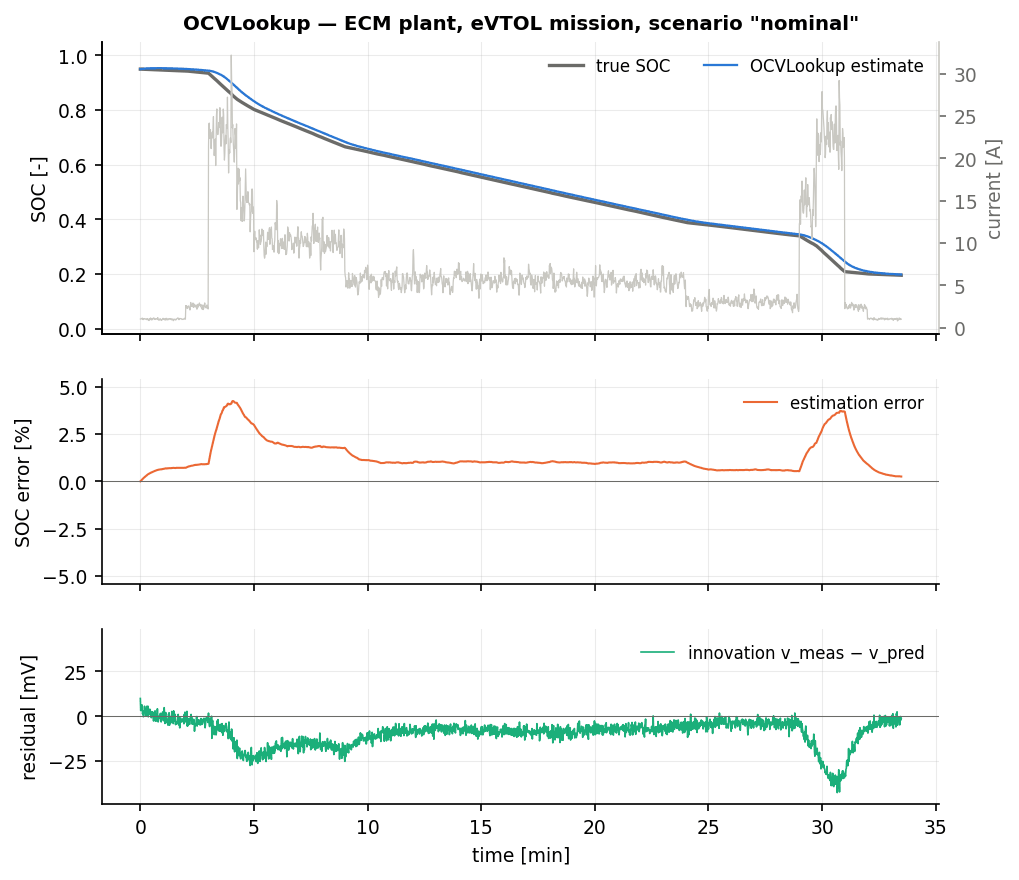
\includegraphics[width=0.78\textwidth]{figures/cell_OCVLookup_nominal.png}
\caption{OCV inversion on the nominal eVTOL mission. The error trace is the low-pass lag
\eqref{eq:ocv-lag}: about $+1\,\%$ through the cruise, rising to $+4\,\%$ during each hover and
decaying with the \SI{30}{\second} filter constant. The residual panel shows the
$-\SI{25}{\milli\volt}$ hover excursions that \eqref{eq:ocv-compensate} fails to remove.}
\end{figure}
\begin{figure}[H]\centering
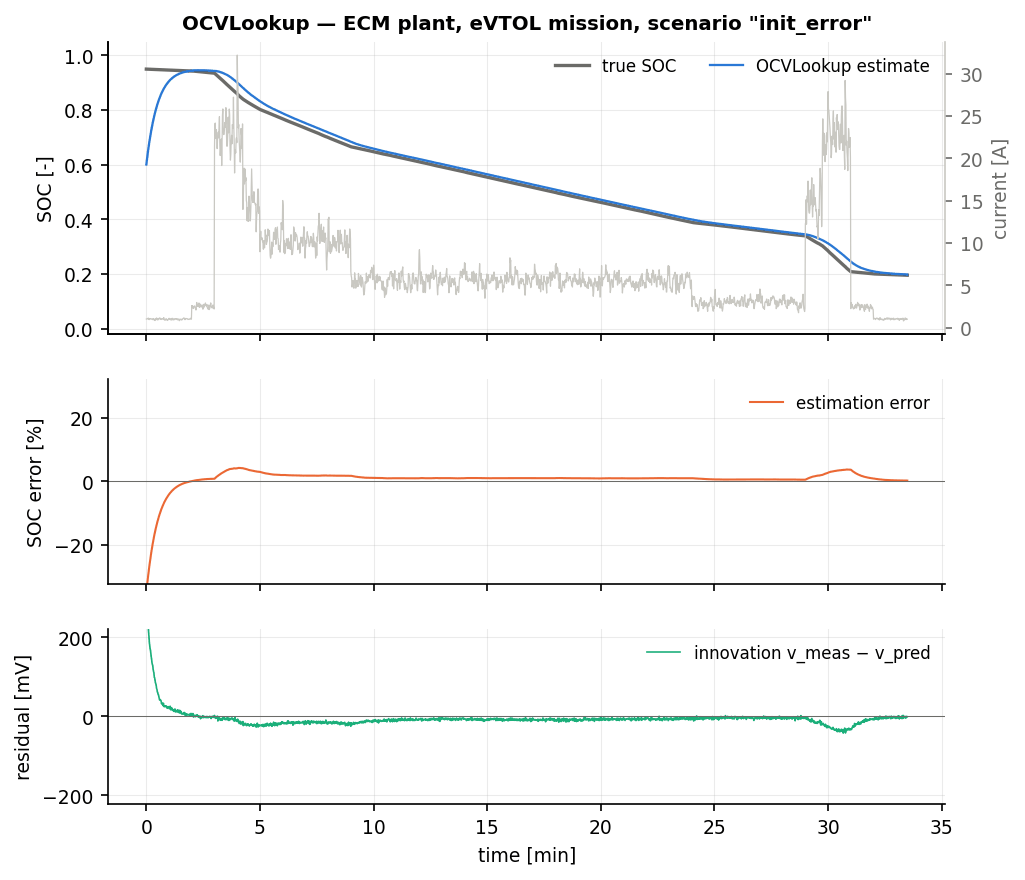
\includegraphics[width=0.78\textwidth]{figures/cell_OCVLookup_init_error.png}
\caption{OCV inversion with a $-35\,\%$ initial SOC error: removed exponentially with the
\SI{30}{\second} constant, after which the trace is indistinguishable from the nominal one. Compare
Chapter~\ref{ch:coulombcounting}, where the same error persists for the whole mission.}
\end{figure}

The headline numbers invert those of Coulomb counting in every respect. On the nominal eVTOL mission
$\text{RMSE}_{\text{ss}} = 1.30\,\%$, nearly four times Coulomb counting's $0.36\,\%$ and
twenty-six times the EKF's $0.05\,\%$; but on \code{init\_error} the steady-state figure is
\emph{also} $1.30\,\%$, with $t_{\text{conv}} = \SI{77}{\second}$ and no divergence, against Coulomb
counting's $35.35\,\%$ and a divergence flag. The method has no memory, so it has no way to be wrong
about the past, and the recovery time predicted by \eqref{eq:ocv-lowpass},
$\tau_{\text{lp}}\ln(0.35/0.02) = \SI{86}{\second}$, brackets the measured value.

The $\text{RMSE}_v$ column sits at \SI{11.7}{\milli\volt} in almost every scenario, against Coulomb
counting's \SI{3.4}{\milli\volt} and the EKF's \SI{0.79}{\milli\volt}. This looks paradoxical for a
method that fits the voltage, and it is the clearest illustration in the report of what
$\text{RMSE}_v$ measures: the method does \emph{not} fit the voltage, it inverts each sample
independently and then filters the result, so the reported state lags and the voltage recomputed
from that lagged state is correspondingly wrong. Fitting and filtering are different operations, and
the EKF is the one that does both at once.

Three scenarios repay a closer look. \code{param\_mismatch} is the method's best column at
$0.41\,\%$ --- three times better than its own nominal result and than the EKF's $1.36\,\%$ --- and
this is a coincidence that should be reported as one: at the cruise current of \SI{5.5}{\ampere},
$R_0\times0.7$ under-compensates the ohmic drop by \SI{19.8}{\milli\volt} while $R_1\times1.3$
over-compensates the fast branch by \SI{9.9}{\milli\volt}, a net $-\SI{9.9}{\milli\volt}$ in
$\widehat{\ocv}$, i.e.\ $-1.2\,\%$ of SOC, which nearly cancels the $+0.9\,\%$ lag of
\eqref{eq:ocv-lag}. Move to a different current and the cancellation disappears.

\code{preisach} is the worst ECM column at $2.15\,\%$ steady-state (whole-run $1.82\,\%$, peak
$4.90\,\%$): the plant's 32-relay operator has a major-loop half-width of \SI{15}{\milli\volt}, with
the charging branch above the discharging branch, against the estimator's $M=\SI{5}{\milli\volt}$,
so $-M\hat h$ removes at most a third of the true hysteresis and does so with the wrong path
dependence. Fifteen to twenty millivolts of uncompensated hysteresis is
\SIrange{1.9}{2.5}{\percent} of SOC at mid-slope, which is the steady-state figure; the peak occurs
on the plateau. Note that the hysteresis is the one term of \eqref{eq:ocv-error} that does not
shrink with current, so it is also what limits the load-gated hybrid of
Chapter~\ref{ch:coulombocvhybrid} ($2.28\,\%$), while Coulomb counting --- which ignores the voltage
--- is unaffected at $0.36\,\%$.

\paragraph{The SPM plant.} On the electrochemical plant the estimators use a 2-RC circuit fitted to
the single-particle model with a \SI{4}{\milli\volt} structured residual (Chapter~\ref{ch:spm}), and
because \eqref{eq:ocv-error} divides the compensation error by the OCV slope, that residual lands
directly on the estimate: $\text{RMSE}_{\text{ss}} = 2.03\,\%$ on \code{nominal} against
$1.30\,\%$ on the ECM plant, and $2.03\,\%$ again on \code{noise\_step}, \code{outliers} and
\code{sensor\_dropout}, since none of those touch the compensation. The degradation is modest
because a \SI{4}{\milli\volt} structural residual is of the same order as the lag term that already
dominates the ECM result. \code{cold} is the outright failure: $6.11\,\%$ steady-state,
$15.29\,\%$ peak, $t_{\text{conv}} = \SI{306}{\second}$, against Coulomb counting's $0.47\,\%$ on
the same data. At \SI{-10}{\celsius} the single-particle model's solid-diffusion overpotential is
large, strongly SOC-dependent and not representable by a constant-parameter 2-RC circuit, so
\eqref{eq:ocv-compensate} is wrong by tens of millivolts and \eqref{eq:ocv-error} converts that
straight into SOC error. When the voltage model breaks down, using the voltage is worse than
ignoring it. The one SPM row that improves on the ECM plant is \code{param\_mismatch} at
$0.60\,\%$ --- the same accidental cancellation as before, now working against a different residual.
Against the EKF the comparison is favourable on \code{nominal} ($2.03\,\%$ versus $3.73\,\%$) and
unfavourable on \code{cold} ($6.11\,\%$ versus $7.35\,\%$ --- both bad), which places OCV inversion
and the EKF in the same band on this plant for the first time: both are limited by the same
measurement model.

\section{Summary}
Use OCV inversion when the estimate must be bounded regardless of history: after a reset, as a
re-initialisation path, as an independent monitor of a drifting primary estimator, or on a duty
cycle with long rests where \eqref{eq:ocv-compensate} reduces to $\widehat{\ocv}\approx v$. Do not
use it as the primary in-flight estimator of a high-power aircraft --- the lag \eqref{eq:ocv-lag} is
\SI{3.75}{\percent} of SOC at hover and cannot be tuned away, the plateau at $\soc\approx0.9$
multiplies every model error by five, and it is more expensive than the EKF that dominates it in ten
of twelve scenarios. Its real contribution is diagnostic: read alongside Coulomb counting it
decomposes the problem into a drift term and a model term, and every filter in Parts~III--X is a
particular compromise between them.

% Copyright 2026 Sreeram Anil
% SPDX-License-Identifier: CC-BY-4.0
% =============================================================================
%  OCV-corrected Coulomb counting under light load — baseline family
% =============================================================================
\chapter{OCV-Corrected Coulomb Counting (Hybrid)}
\label{ch:coulombocvhybrid}

\section*{At a glance}
\begin{tabular}{@{}l>{\raggedright\arraybackslash}p{0.76\textwidth}@{}}
Family & baselines \\
Header & \texttt{include/estkit/battery/baselines.hpp} \\
Registered name & \texttt{CoulombOCVHybrid} \\
State dimension & $n_x = 4$ propagated open-loop; $\soc$ corrected while $\abs{i} < 0.3\,$C \\
Options & \code{i\_thr\_C} $=0.3$, \code{tau\_corr} $=\SI{60}{\second}$ \\
Cost per step & $\mathcal{O}(n_x)$ under load, $+\,n_b=40$ bisection steps when correcting; $\approx 211$\,ns/step \\
Primary references & \cite{ng2009coulomb,plett2015bms1,hu2012comparative} \\
\end{tabular}

\section{Motivation and relevance}
Chapters~\ref{ch:coulombcounting} and~\ref{ch:ocvlookup} established a clean complementarity.
Ampere-hour integration is smooth, cheap and drift-prone, and its error
\eqref{eq:cc-drift} grows without bound. Open-circuit-voltage inversion is bounded and
memoryless, but under load its accuracy is set by how well the overpotential
$R_0 i + v_1 + v_2 - Mh$ --- several hundred millivolts during a hover --- is modelled, and the
low-pass it needs to reject noise converts the SOC rate into a lag of
\SI{3.75}{\percent} \eqref{eq:ocv-lag}.

Both objections to the voltage inversion vanish at \emph{low current}: the overpotential to be
compensated shrinks in proportion to $i$, so a \SI{10}{\percent} error in $R_0$ costs
\SI{1.2}{\milli\volt} at \SI{1}{\ampere} instead of \SI{27}{\milli\volt} at \SI{22.5}{\ampere}, and
the lag term $\tau i/(3600Q)$ shrinks with it. The engineering response --- and what most shipped
battery-management systems implement in one form or another --- is therefore to integrate at all
times and to \emph{pull the count towards the voltage-derived SOC whenever the load is light enough
for that SOC to be trustworthy}: the cheapest possible approximation to a Kalman filter, a gain that
is zero above a current threshold and a fixed first-order constant below it, scheduled on the
measured current instead of computed from a covariance.

The interest for an electric aircraft is that this is the only baseline that is both drift-corrected
\emph{and} usable in flight. It does not require the cell to rest --- an eVTOL mission contains no
rest at all --- only that the mission contain phases at a fraction of the cruise current, which
preflight checks and postflight shutdown do provide: about \SI{10}{\percent} of every profile in the
benchmark (\S\ref{sec:hy-duty}).

\section{Problem statement}
The method estimates $\soc$ by \eqref{eq:cc-recursion} and applies a correction whenever the
measured current is below a threshold.
\begin{assumption}\label{as:hy-all}
(i) Below $i_{\text{thr}}$, the compensated open-circuit voltage \eqref{eq:ocv-compensate} is an
unbiased proxy for $\ocv(\soc,T)$ --- that is, the residual model error at low current is small
compared with the accuracy required; (ii) the mission contains enough time below $i_{\text{thr}}$
for a first-order correction of time constant $\tau_{\text{corr}}$ to act.
\end{assumption}
Assumption~(i) fails for the hysteresis, which does \emph{not} shrink with current, and for the
SPM plant at low temperature; assumption~(ii) is a property of the duty cycle, quantified in
\S\ref{sec:hy-duty}.

\section{Derivation}

\subsection{The blended update}
Each sample performs the open-loop time update of the full four-state model --- Coulomb counting on
$\soc$, and the RC and hysteresis states driven by the measured current --- and then, conditionally,
a correction on $\soc$ alone:
\begin{align}
\xhat_k &= f(\xhat_{k-1}, \vu_{k-1}), \label{eq:hy-predict}\\
\widehat{\ocv}_k &= v^{\text{m}}_k + R_0(T^{\text{m}}_k)\,i^{\text{m}}_k
 + \hat v_{1,k} + \hat v_{2,k} - M\,\hat h_k, \label{eq:hy-proxy}\\
\hat\soc_k &\gets a\,\hat\soc_k + (1-a)\,\ocv^{-1}\!\bigl(\widehat{\ocv}_k, T^{\text{m}}_k\bigr),
 \qquad a = e^{-\dt/\tau_{\text{corr}}},
 \qquad\text{if } \abs{i^{\text{m}}_k} < i_{\text{thr}}, \label{eq:hy-correct}
\end{align}
with $i_{\text{thr}} = 0.3\,Q_{\text{nom}}/\si{\hour} = \SI{1.5}{\ampere}$ for the
\SI{5}{\ampere\hour} cell and $\tau_{\text{corr}} = \SI{60}{\second}$, so
$a = e^{-0.1/60} = 0.998334$. The inversion $\ocv^{-1}$ is the same 40-step bisection on
$[-0.05,1.05]$ used in Chapter~\ref{ch:ocvlookup}; the compensation \eqref{eq:hy-proxy} is
also identical, so the method is exactly ``Coulomb counting, dragged towards \code{OCVLookup}'s
instantaneous estimate at a rate $1/\tau_{\text{corr}}$, but only while the load is light''.

Two structural points distinguish it from the rest-based re-anchoring of ground-vehicle practice: it
never waits (there is no rest timer and no dwell, so the correction begins on the first light-load
sample), and the RC states are \emph{compensated} rather than assumed decayed, so the
overpotentials need not be zero --- only small enough that the model's error in them is tolerable.

\subsection{Error dynamics}
Let $e_k = \hat\soc_k - \soc_k$ and let $e^{\ocv}$ denote the error of the voltage-derived SOC
itself, which by \eqref{eq:ocv-error} is the compensated-voltage error divided by the OCV slope.
Combining \eqref{eq:cc-drift} with \eqref{eq:hy-correct}, the error obeys a \emph{switched} linear
recursion: in continuous-time form,
\begin{equation}
\dot e \;=\;
\begin{cases}
\;\;\dot e_{\text{drift}}, & \abs{i} \ge i_{\text{thr}} \quad\text{(open loop)},\\[4pt]
-\dfrac{1}{\tau_{\text{corr}}}\bigl(e - e^{\ocv}\bigr) \;+\; \dot e_{\text{drift}},
 & \abs{i} < i_{\text{thr}} \quad\text{(corrected)},
\end{cases}
\label{eq:hy-switched}
\end{equation}
where $\dot e_{\text{drift}}$ is the instantaneous version of the gain, offset and capacity terms of
\eqref{eq:cc-drift}. Over a single light-load window $[t_0,t_1]$ of duration $T_w$, and neglecting
the drift accumulated within it (at $\abs{i}<\SI{1.5}{\ampere}$ it is at most
\SI{0.02}{\percent} of SOC per minute), \eqref{eq:hy-switched} integrates to
\begin{equation}
\boxed{\;
e(t_1) \;=\; e^{\ocv} \;+\; \bigl(e(t_0) - e^{\ocv}\bigr)\,e^{-T_w/\tau_{\text{corr}}} \;}
\label{eq:hy-window}
\end{equation}
so each light-load window contracts whatever error the estimator is carrying by the factor
$e^{-T_w/\tau_{\text{corr}}}$, towards a floor $e^{\ocv}$ that the correction cannot go below.
Three consequences follow, and between them they explain every row of the results table.

\paragraph{The error is reduced, never removed, and only in bursts.} An initial error survives a
mission in proportion to the \emph{total} light-load time: with windows $T_{w,1},T_{w,2},\dots$ the
surviving fraction is $\exp\bigl(-\sum_j T_{w,j}/\tau_{\text{corr}}\bigr)$. Between windows the
estimate is pure Coulomb counting and the error is frozen at whatever the last window left. This is
visible as a staircase in the error trace and is the defining signature of the method.

\paragraph{The floor is the low-current OCV error.} $e^{\ocv}$ is what
Chapter~\ref{ch:ocvlookup} measures, evaluated at $\abs{i}<i_{\text{thr}}$ rather than at the hover
current, and with a much smaller lag: $\tau_{\text{corr}}\,i/(3600Q) = \SI{0.33}{\percent}$ at
\SI{1}{\ampere} against \SI{3.75}{\percent} for \code{OCVLookup} at hover. The two terms of
\eqref{eq:ocv-error} that do \emph{not} shrink with current are the voltage-sensor error and the
hysteresis mismatch $M\,\delta h$, and the latter therefore sets the floor: with
$M = \SI{5}{\milli\volt}$ and an estimator that initialises $\hat h_0 = 0$ while the plant arrives
from a charge at $h=+1$, the proxy is biased by \SI{5}{\milli\volt}, i.e.\
$5/800 = \SI{0.6}{\percent}$ of SOC at mid-slope.

\paragraph{The threshold is a duty-cycle decision, not a tuning knob.} $i_{\text{thr}}$ decides
which mission segments contribute at all, and because a profile is a staircase in current, the map
from $i_{\text{thr}}$ to correction time is a step function.

\subsection{How much light load does a mission contain?}
\label{sec:hy-duty}
Counting the samples with $\abs{i^{\text{m}}}<\SI{1.5}{\ampere}$ in each benchmark profile
(seed~1, nominal sensors) gives:

\begin{table}[H]\centering\small
\caption{Light-load duty of the benchmark profiles at $i_{\text{thr}} = 0.3\,$C
($\SI{1.5}{\ampere}$), and the resulting contraction factor
$\exp(-\sum T_w/\tau_{\text{corr}})$ applied to any error the estimator carries into the mission.}
\label{tab:hy-duty}
\begin{tabular}{@{}lrrrr@{}}\toprule
profile & mission [\si{\second}] & light load [\si{\second}] & fraction & $\sum T_w/\tau_{\text{corr}}$ \\ \midrule
\code{evtol}          & 2010 & 210.0 & \SI{10.4}{\percent} & 3.50 \\
\code{fixed\_wing}    & 2880 & 331.6 & \SI{11.5}{\percent} & 5.53 \\
\code{hover\_hold}    & 1140 & 120.0 & \SI{10.5}{\percent} & 2.00 \\
\code{ground\_charge} & 3600 & 526.0 & \SI{14.6}{\percent} & 8.77 \\
\bottomrule\end{tabular}
\end{table}

For the eVTOL mission the light-load time is exactly the \SI{120}{\second} \code{preflight} and the
\SI{90}{\second} \code{postflight} segments, both at 0.20\,C $=\SI{1.0}{\ampere}$; \code{taxi} at
0.50\,C $=\SI{2.5}{\ampere}$ is excluded, and so is everything else. The threshold choice is what
makes those two segments count: at $i_{\text{thr}} = 0.2\,$C nothing in the mission would qualify,
and at $0.55\,$C the two taxi segments would be added. \code{fixed\_wing} is the interesting case:
its \code{descent} segment sits at exactly 0.30\,C, so with a \SI{15}{\percent} gust fraction it
straddles the threshold and contributes about \SI{150}{\second} of intermittent, chattering
correction --- a reminder that a hard threshold on a noisy signal is a switching surface, and that a
production implementation should hysteresis-band it.

\section{Algorithm}
\begin{algorithm}[H]
\caption{OCV-corrected Coulomb counting --- one sampling period}
\begin{algorithmic}[1]
\Require $\xhat_{k-1}$, stored $\vu_{k-1}$, new $i^{\text{m}}_k, v^{\text{m}}_k, T^{\text{m}}_k$
\State $\vu_k \gets [\,i^{\text{m}}_k,\ T^{\text{m}}_k\,]^\T$
\If{$k>0$} \State $\xhat_k \gets f(\xhat_{k-1},\vu_{k-1})$ \Comment{ampere-hour integration plus open-loop $v_1,v_2,h$}
\EndIf
\State $\hat v_k \gets h(\xhat_k,\vu_k)$ \Comment{prior voltage prediction, for the residual metric}
\If{$\abs{i^{\text{m}}_k} < i_{\text{thr}}$}
 \State $\widehat{\ocv} \gets v^{\text{m}}_k + R_0(T^{\text{m}}_k)\,i^{\text{m}}_k + \hat v_1 + \hat v_2 - M\hat h$
 \State $\soc^{\ocv} \gets$ \textbf{bisect} $\ocv(\cdot,T^{\text{m}}_k) = \widehat{\ocv}$ on $[-0.05,1.05]$, 40 steps
 \State $\xhat_k[\soc] \gets a\,\xhat_k[\soc] + (1-a)\,\soc^{\ocv}$, \quad $a = e^{-\dt/\tau_{\text{corr}}}$
\EndIf
\State $\vu_{k-1}\gets\vu_k$
\Ensure $\hat\soc_k = \xhat_k[\soc]$
\end{algorithmic}
\end{algorithm}
Note that only $\soc$ is corrected: $v_1, v_2, h$ continue to be propagated open-loop from the
measured current, so an error in the hysteresis state is never removed and feeds
\eqref{eq:hy-proxy} as a persistent bias for the whole mission.

\section{Application and implementation notes}
The two options are fixed for every scenario at \code{i\_thr\_C} $=0.3$ and \code{tau\_corr}
$=\SI{60}{\second}$; the threshold is expressed as a C-rate so that it scales with the cell, and
\SI{60}{\second} is short enough to act within a \SI{120}{\second} preflight (two time constants)
and long enough to average the \SI{2}{\milli\volt} sensor noise down to
$\SI{0.25}{\percent}\times\sqrt{\dt/2\tau_{\text{corr}}} = \SI{0.007}{\percent}$ of SOC.

At \SI{211}{\nano\second} per step the method sits between Coulomb counting
(\SI{79}{\nano\second}) and \code{OCVLookup} (\SI{1310}{\nano\second}), exactly as the duty cycle
predicts: the expensive bisection runs on about \SI{10}{\percent} of the samples, so the average cost
is $79 + 0.104\times(1310-79) \approx \SI{207}{\nano\second}$. That agreement is reassuring but it is
also the method's one embedded-systems liability --- the execution time is \emph{data-dependent}, so
a worst-case timing analysis must budget the full \SI{1310}{\nano\second} for every sample, since a
mission flown entirely at low current would take the branch every time. This is the only estimator
in the baseline family that violates the determinism property of \S\ref{sec:lib-mcu}. \code{sizeof}
is \SI{4192}{\byte}, essentially all OCV table, and the float32 build is unaffected: there is no
covariance to lose definiteness and the correction is a convex combination of bounded quantities.

\section{Benchmark results}
\label{sec:hy-results}
% Copyright 2026 Sreeram Anil
% SPDX-License-Identifier: CC-BY-4.0
\begin{table}[H]\centering\footnotesize\setlength{\tabcolsep}{4pt}
\caption{CoulombOCVHybrid: cell-level benchmark on the eVTOL mission (mean over seeds; RMSE and max error in \% SOC; $t_\mathrm{conv}$: first time the error stays below 2\,\% for 60\,s, -- = never; EKF reference: steady-state RMSE of the plain EKF on the same data).}\label{tab:cell_CoulombOCVHybrid}
\begin{tabular}{llrrrrrcrr}\toprule
plant & scenario & RMSE & RMSE$_\mathrm{ss}$ & max & $t_\mathrm{conv}$ [s] & RMSE$_v$ [mV] & div. & EKF ref. & ns/step \\ \midrule
ECM & nominal & 0.28 & 0.17 & 0.50 & 0 & 1.79 & no & 0.05 & 211 \\
ECM & init\_error & 5.97 & 4.42 & 34.94 & -- & 46.91 & no & 0.05 & 211 \\
ECM & current\_bias & 1.44 & 1.94 & 2.87 & 0 & 18.50 & no & 0.61 & 211 \\
ECM & noise\_step & 0.28 & 0.17 & 0.50 & 0 & 1.80 & no & 0.12 & 209 \\
ECM & outliers & 0.14 & 0.05 & 0.35 & 0 & 1.40 & no & 0.21 & 209 \\
ECM & cold & 0.35 & 0.21 & 0.60 & 0 & 2.59 & no & 0.16 & 208 \\
ECM & hot & 0.31 & 0.24 & 0.47 & 0 & 2.43 & no & 0.03 & 210 \\
ECM & aged\_cell & 7.37 & 9.41 & 12.65 & 0 & 105.00 & no & 1.52 & 209 \\
ECM & param\_mismatch & 0.13 & 0.16 & 0.47 & 0 & 17.14 & no & 1.36 & 210 \\
ECM & sensor\_dropout & 0.28 & 0.17 & 0.50 & 0 & 1.79 & no & 0.46 & 210 \\
ECM & preisach & 2.20 & 2.28 & 2.44 & 0 & 22.75 & no & 0.20 & 209 \\
ECM & combined & 3.23 & 1.33 & 24.96 & 252 & 35.68 & no & 12.44 & 211 \\
\midrule
SPM & nominal & 0.55 & 0.66 & 0.82 & 0 & 10.80 & no & 3.73 & 206 \\
SPM & init\_error & 6.60 & 5.23 & 34.94 & -- & 52.85 & no & 3.81 & 205 \\
SPM & current\_bias & 2.21 & 2.90 & 3.94 & 0 & 26.81 & no & 5.69 & 205 \\
SPM & noise\_step & 0.55 & 0.66 & 0.82 & 0 & 10.82 & no & 3.30 & 205 \\
SPM & outliers & 0.72 & 0.83 & 0.98 & 0 & 11.55 & no & 1.99 & 205 \\
SPM & cold & 3.39 & 3.50 & 3.71 & -- & 50.59 & no & 7.35 & 205 \\
SPM & hot & 0.37 & 0.46 & 0.61 & 0 & 8.85 & no & 2.16 & 205 \\
SPM & param\_mismatch & 0.88 & 0.99 & 1.16 & 0 & 15.97 & no & 3.13 & 205 \\
SPM & sensor\_dropout & 0.55 & 0.66 & 0.82 & 0 & 10.80 & no & 5.31 & 207 \\
\bottomrule\end{tabular}\end{table}

\begin{figure}[H]\centering
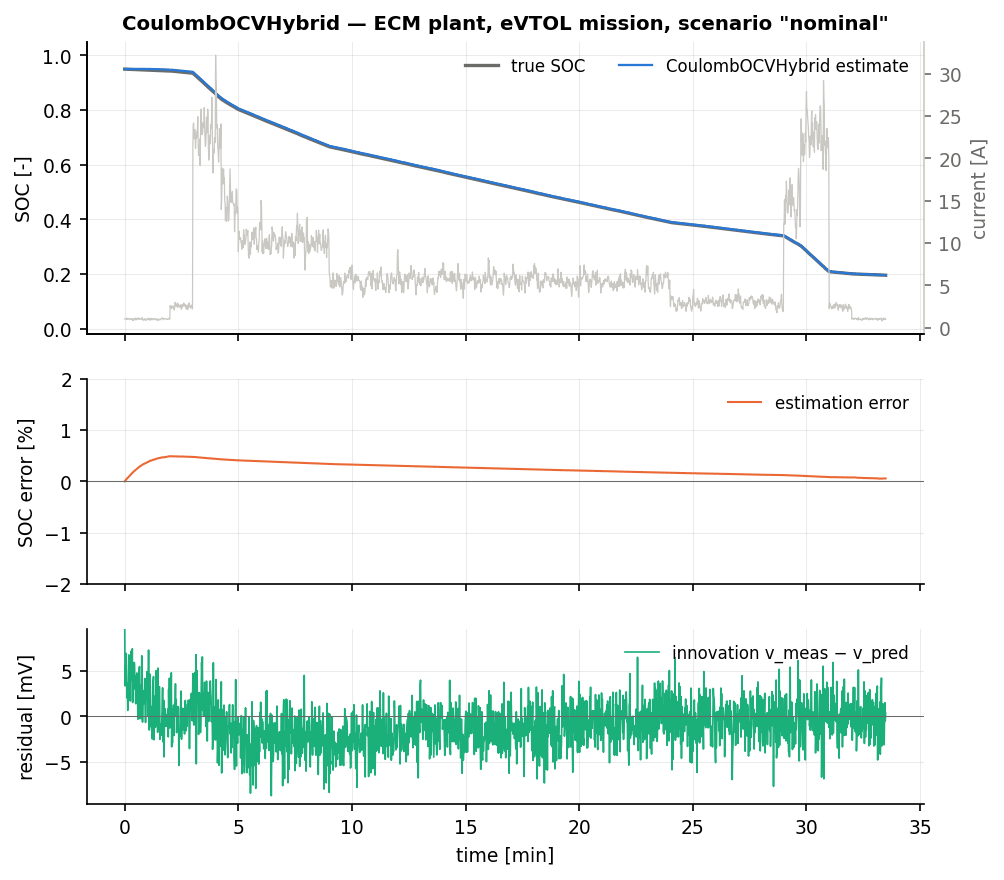
\includegraphics[width=0.78\textwidth]{figures/cell_CoulombOCVHybrid_nominal.png}
\caption{The hybrid on the nominal eVTOL mission. The error rises to $+0.47\,\%$ during the
\SI{120}{\second} preflight as the correction pulls the count towards a proxy biased by the
uninitialised hysteresis state, holds through the flight as pure Coulomb counting, and is pulled
back towards zero during the \SI{90}{\second} postflight.}
\end{figure}
\begin{figure}[H]\centering
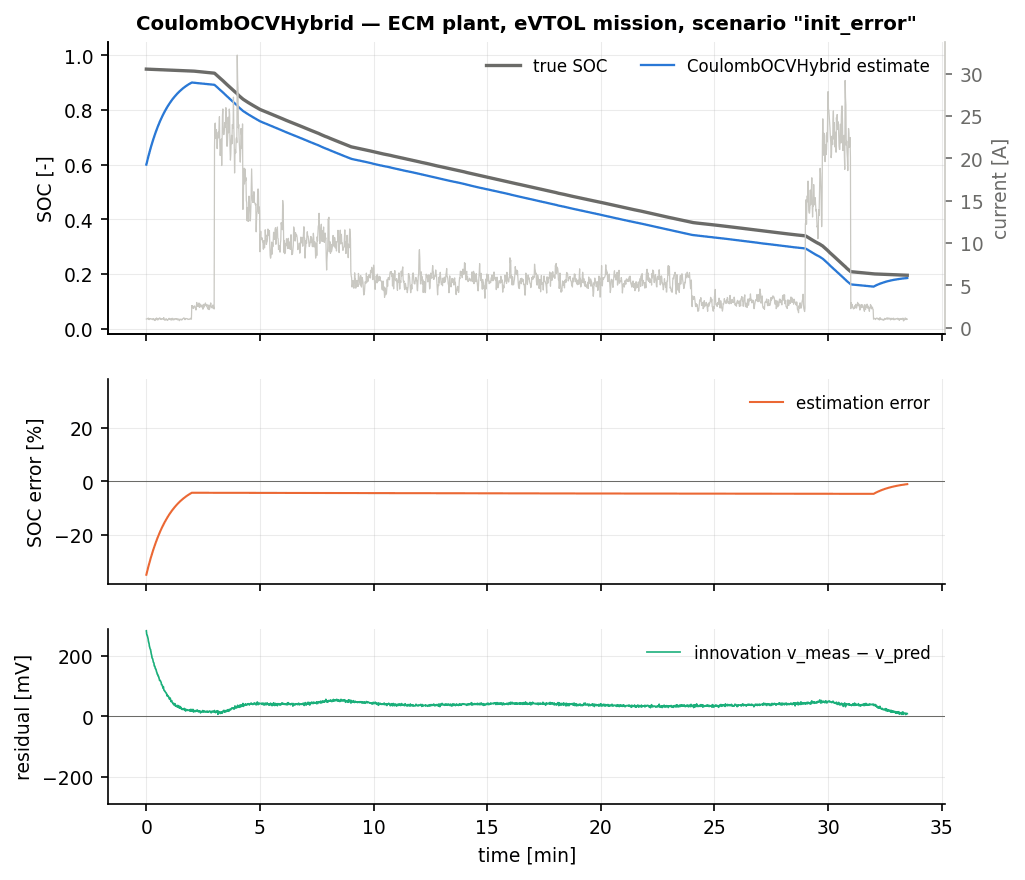
\includegraphics[width=0.78\textwidth]{figures/cell_CoulombOCVHybrid_init_error.png}
\caption{The hybrid with a $-35\,\%$ initial SOC error. Two time constants of preflight correction
contract it to $-4.4\,\%$ by $t=\SI{2}{\minute}$; the error is then frozen for the whole flight and
contracted again to about $-1\,\%$ during the postflight --- the staircase predicted by
\eqref{eq:hy-window}. Compare Chapter~\ref{ch:coulombcounting}, where the same error persists
undiminished.}
\end{figure}

\paragraph{Nominal.} $\text{RMSE}_{\text{ss}} = 0.17\,\%$ against Coulomb counting's $0.36\,\%$ and
\code{OCVLookup}'s $1.30\,\%$: the hybrid is better than either of its parents, which is the whole
point of the construction. The voltage-residual RMSE drops from \SI{3.41}{\milli\volt} to
\SI{1.79}{\milli\volt} for the same reason. The residual $0.17\,\%$ is not the Coulomb-counting
drift but the floor $e^{\ocv}$ of \eqref{eq:hy-window}: the error trace peaks at $+0.47\,\%$ during
preflight --- close to the \SI{0.6}{\percent} that a \SI{5}{\milli\volt} hysteresis bias predicts at
mid-slope --- and then decays as the drift of \eqref{eq:cc-drift}, which has the opposite sign,
works against it. Note the sign inversion relative to Coulomb counting, whose nominal error is
$-0.44\,\%$: the two methods fail in opposite directions.

\paragraph{Initial error.} $\text{RMSE}_{\text{ss}} = 4.42\,\%$ against Coulomb counting's
$35.35\,\%$, with the divergence flag cleared. Equation~\eqref{eq:hy-window} with
$T_w = \SI{120}{\second}$ predicts $35\times e^{-2} = 4.7\,\%$ surviving the preflight window, which
is what the trace holds for the rest of the flight; the postflight window contracts it by a further
$e^{-1.5} = 0.22$. The convergence criterion still reports ``--'', because the error only falls
below \SI{2}{\percent} in the final minute and never sustains it for the required
\SI{60}{\second} --- an honest reading: a $35\,\%$ prior error is \emph{survived}, not removed.

\paragraph{Faults on the current channel.} \code{current\_bias} gives $1.94\,\%$ against Coulomb
counting's $3.20\,\%$, and \code{combined} $1.33\,\%$ against $20.94\,\%$ --- a factor of sixteen,
and the largest single improvement in the baseline part. In \code{combined} the correction removes
most of the $-25\,\%$ prior during preflight and then re-anchors after the landing hover, so the
convergence criterion is met at $t=\SI{252}{\second}$ where Coulomb counting never converges. The
remaining $1.33\,\%$ is the flight-phase drift of a \SI{0.15}{\ampere} bias and a \SI{10}{\percent}
capacity error accumulating unchecked between the two windows. \code{aged\_cell} improves only
marginally ($9.41\,\%$ against $10.05\,\%$): the capacity error is a \emph{rate}, so it regenerates
during the \SI{30}{\minute} of open-loop flight faster than \SI{210}{\second} of correction can
remove it. That contrast --- a bias is removed, a rate is not --- is the sharpest statement of what
a periodically-corrected integrator can and cannot do.

\paragraph{Faults on the voltage channel.} These now matter, because the voltage is used.
\code{noise\_step} and \code{sensor\_dropout} are both unchanged from nominal at $0.17\,\%$, for the
same reason in both cases: the voltage step at $t=\SI{600}{\second}$ and the \SI{15}{\second}
dropout from $t=\SI{200}{\second}$ both fall inside high-current segments, where the correction is
switched off. The method is accidentally immune to any voltage fault that occurs in flight --- a
genuine robustness property of load gating, and a fragile one, since a fault during preflight would
be adopted directly. \code{outliers} scores $0.05\,\%$, better than nominal, because the
$\pm\SI{50}{\milli\volt}$ outliers are zero-mean, the \SI{60}{\second} correction averages them
away, and the extra noise happens to perturb the proxy against the hysteresis bias --- a coincidence
of one seed set, not a property.

\paragraph{Hysteresis.} \code{preisach} is the method's worst ECM scenario at
$\text{RMSE}_{\text{ss}} = 2.28\,\%$, against $0.36\,\%$ for Coulomb counting, which ignores the
voltage entirely, and $0.20\,\%$ for the EKF. The mechanism is \eqref{eq:hy-proxy}: the plant's
32-relay Preisach operator has a major-loop half-width of \SI{15}{\milli\volt} with the charging
branch above the discharging branch, while the estimator subtracts only $M\hat h$ with
$M = \SI{5}{\milli\volt}$ from an $\hat h$ that is itself propagated open-loop. The proxy is
therefore biased by \SIrange{15}{20}{\milli\volt}, and \eqref{eq:ocv-error} converts that to
\SIrange{1.9}{2.5}{\percent} of SOC at mid-slope. This is the characteristic failure of the whole
design: the correction is only as good as the OCV proxy, and it imports the proxy's bias with full
weight. Coulomb counting is \emph{better} here precisely because it declines to look.
\code{param\_mismatch} ($0.16\,\%$), by contrast, is essentially unaffected --- the $R_0$ and $R_1$
errors are multiplied by \SI{1}{\ampere} during the correction windows and contribute under
\SI{4}{\milli\volt}.

\paragraph{The SPM plant.} On the electrochemical plant the estimators are given a 2-RC circuit
fitted to it with a \SI{4}{\milli\volt} structured residual (Chapter~\ref{ch:spm}), and the hybrid
inherits that residual through its proxy: $\text{RMSE}_{\text{ss}} = 0.66\,\%$ on \code{nominal},
against $0.47\,\%$ for Coulomb counting and $2.03\,\%$ for \code{OCVLookup}. The ordering is the
informative part. The hybrid is \emph{worse} than pure integration, because it injects a biased
voltage estimate into an otherwise unbiased count; but it is three times \emph{better} than pure
inversion, because it only does so at \SI{1}{\ampere}, where the SPM's Butler--Volmer and diffusion
overpotentials are smallest, and because the \SI{60}{\second} correction is much shorter than
\code{OCVLookup}'s permanent \SI{30}{\second} lag applied at hover currents. The \code{cold} row
makes the same point at the limit: at \SI{-10}{\celsius} the SPM's diffusion impedance is not
representable by the fitted circuit at all, the proxy is wrong by tens of millivolts even at
\SI{1}{\ampere}, and the hybrid degrades to $3.50\,\%$ with the convergence criterion never met,
while Coulomb counting scores $0.47\,\%$. Elsewhere on the SPM plant the pattern of the ECM rows
survives: \code{current\_bias} $2.90\,\%$ improves on Coulomb counting's $3.31\,\%$,
\code{init\_error} contracts $35\,\%$ to $5.23\,\%$, and \code{hot} ($0.46\,\%$) is the best row of
all because the higher temperature both shrinks the overpotential and speeds the kinetics the fitted
circuit gets wrong. With the single exception of \code{init\_error} --- where the EKF's covariance
lets it absorb the prior error in one sample and score $3.81\,\%$ against the hybrid's $5.23\,\%$
--- every one of these rows beats the EKF's own SPM figures (\numrange{3.73}{7.35}\,\%). That is the
recurring surprise of the SPM columns: when the measurement model carries a structured error, a
method that uses the measurement sparingly does better than one that trusts it every sample.

\section{Summary}
Use load-gated OCV correction whenever the duty cycle spends even a few per cent of its time at a
fraction of the cruise current, which almost every real mission does --- it costs
\SI{211}{\nano\second} per step, removes a $35\,\%$ prior error down to $4.4\,\%$, cuts the
\code{combined} scenario by a factor of sixteen against plain Coulomb counting, and is the best of
the three baselines on seven of the twelve ECM scenarios (tied with Coulomb counting on an
eighth, \code{hot}). Size the threshold from the mission's current
staircase rather than by tuning, band it with hysteresis so that a segment sitting on the threshold
does not chatter, and choose $\tau_{\text{corr}}$ so that the shortest useful window is two or three
time constants. Do not use it where the OCV proxy is biased rather than noisy --- unmodelled
hysteresis (\code{preisach}, $2.28\,\%$) and structured electrochemical model error at low
temperature (SPM \code{cold}, $3.50\,\%$) are both imported at full weight --- and do not expect it
to track a \emph{drifting} capacity, because \code{aged\_cell} shows that a rate regenerates between
correction windows faster than the windows can remove it. Its real lesson for the rest of this
report is structural: it is a Kalman filter with the gain replaced by a hand-set schedule, and every
one of its failures is a case where a covariance would have told the estimator how much to trust the
measurement.

